\subsection{Test-case generation algorithm}

\begin{figure}
\centering
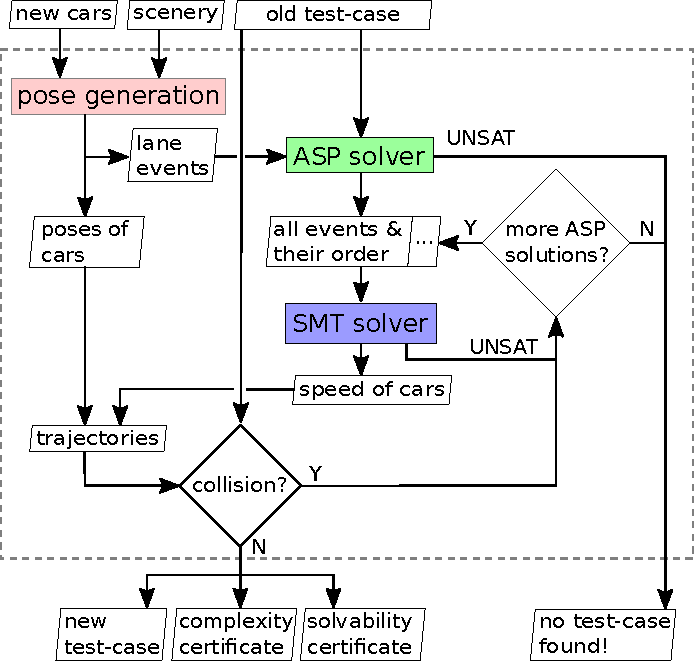
\includegraphics[width=85mm]{figures/chapter4/algorithm.pdf}%
\caption{The test-case generation algorithm.}
\label{fig:algorithm}%
\end{figure}

Our algorithm has three main steps.
%
These steps are highlighted with red, green and blue in Figure~\ref{fig:algorithm}.

%---------------------
\subsubsection{Step 1: pose generation}
The first step is to determine the poses of each car such that they satisfy the car's \emph{steering constraints}.
%
Two consecutive poses $p_1, p_2$ at times $t_1, t_2$ respectively, satisfy the constraint if and only if there exists a steering input as a function of time over the interval $[t_1, t_2]$ that drives the car from $p_1$ to $p_2$.
%
Note that a pose specifies both the location and the orientation of the car.
%
The constraint depends on the steering mechanism of each car e.g. steering axles, maximum steering angles, wheelbase, etc.

%---simulation
The algorithm drives each car using a steering controller in a physics simulation, so the generated pose-sequence satisfies the steering constraints.
%
The steering controller tracks the centerline of the car's route.
%
A speed controller is used to track a constant speed.
%
See Figure~\ref{fig:sim-pose} for a pose sequence.
%
A location is shown by a dot and the orientation is implied by the tangent to the dot sequence.

%---success
If the two ego trajectories (candidates for complexity and solvability certificates) reach ego's goal, our algorithm proceeds to Step 2.
%
Note that the new non-egos do not need to reach their goal.

%---failure
Otherwise, the algorithm stops and returns with failure.
%
If we have a solvability certificate for the old test-case, we can simply use its poses and skip the simulations of ego, so Step 1 would not fail.

\begin{figure}
\centering
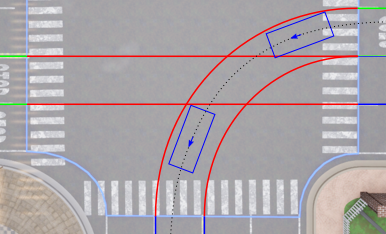
\includegraphics[width=60mm]{figures/chapter4/sim-poses-landscape.png}%
\caption{Two poses at which lane events happen are shown with arrows, and the car's shape with rectangles.}
\label{fig:sim-pose}%
\end{figure}


%-----------second step----------
\subsubsection{Step 2: deciding order of events}
This step finds all possible order of events such that one of the ego behaviors would qualify as a complexity certificate, and the other as a solvability certificate.
%
The set of events and their perceptible order affect the traffic rules violations.
%
Some of this information is already fixed by the behavior of old non-egos.
%
The lane events of each new car are computed from its pose sequence from Step 1, the car's shape, and scenery's lane geometry.
%
Furthermore, for each car, the temporal order between its lane events are implied by the poses at which they happen and the order between poses in the sequence.
%
Each event is assigned a symbolic time such that simultaneous lane events are assigned the same time symbol.
%
It remains to determine what stop events should happen and what is the perceptible order between all events.

%---CSP
Therefore, this step is a CSP where the \emph{search variables} are the stop events and the perceptible order between events.
%
The search space is finite since there are only a finite number of events and possible order between them.
%
The \emph{constraints} include the old events and their temporal and perceptible order, the new lane events and their temporal order, and
the complexity and solvability criteria.
%
Our algorithm specifies this search problem as an ASP program and solves it with an ASP solver.



%---perceptible order 
The perceptible order between time symbols is represented by two binary relations  \clingo{equal()} and \clingo{lessThan()}.
%
If we instruct the ASP solver to make a choice about the perceptible order of every pair of time symbols, we make the search space unnecessarily big.
%
Instead, we manually go through the set of traffic rules and add a choice rule only for each pair of events that their perceptible order matters to the right-of-way violations.
%
This manual derivation has to be done only once for each traffic rule, say after modeling the traffic rules for an intersection.
%
For example, consider the traffic rule 
\begin{quote}
``The driver of a vehicle approaching an intersection shall yield the right-of-way
to any vehicle which has entered the intersection from a different highway,''    
\end{quote}
and its ASP encoding
\begin{minted}[fontsize=\small]{prolog}
violatesRightOfForRule(V1, V2, yieldToInside):-
  enteredForkAtTime(V1, F1, Te1),
  enteredForkAtTime(V2, F2, Te2),
  onDifferentHighways(F1, F2),
  requestedLane(V1, L1), requestedLane(V2, L2),
  overlaps(L1, L2),
  lessThan(Te2, Te1),
  leftLaneAtTime(V2, L1, T1),
  enteredLaneAtTime(V1, L2, T2),
  lessThan(T2, T1).
\end{minted}
%
For this rule, we only need a choice for \clingo{lessThan(Te2, Te1)}:
\begin{minted}[fontsize=\small]{prolog}
{equal(Te1,Te2); lessThan(Te1,Te2); lessThan(Te2,Te1)}=1 :- 
  enteredForkAtTime(V1, F1, Te1),
  enteredForkAtTime(V2, F2, Te2),
  onDifferentHighways(F1, F2), 
  requestedLane(V1, L1), requestedLane(V2, L2),
  overlaps(L1, L2).
\end{minted}
and a choice for \clingo{lessThan(T2, T1)}:
\begin{minted}[fontsize=\small]{prolog}
{equal(T1, T2); lessThan(T1, T2); lessThan(T2, T1) } = 1 :-
  enteredForkAtTime(V1, F1, Te1),
  enteredForkAtTime(V2, F2, Te2),
  onDifferentHighways(F1, F2),
  requestedLane(V1, L1), requestedLane(V2, L2),
  overlaps(L1, L2),
  lessThan(Te2, Te1),
  leftLaneAtTime(V2, L1, T1),
  enteredLaneAtTime(V1, L2, T2).
\end{minted}

%---temporal order
Temporal order is different from perceptible order as discussed earlier.
%
The temporal order between time symbols is represented using a binary relation \clingo{realLTE()}.
%
The `LTE' stands for Less-Than-or-Equal-to and emphasizes that the binary relation is a partial order (and so transitive).
%
The `real' emphasizes the intended meaning of this relation as the order between real numbers.
%
The order between real numbers is total but  \clingo{realLTE()} is partial, since the temporal order between lane events of two different cars are not physically constrained and may not matter to traffic rules violations either.
%
In particular, time symbols \clingo{s,t} are simultaneous if and only if
\clingo{realLTE(s,t)} and \clingo{realLTE(t,s)}, \clingo{s} precedes \clingo{t} if and only if 
\clingo{realLTE(s,t)} and \clingo{not realLTE(t,s)}, and the order is unknown (and unimportant) if and only if \clingo{not realLTE(s,t)} and \clingo{not realLTE(t,s)}.
%
For each new car, the temporal order between its lane events are already determined by Step 1, and are added as facts to the ASP program.

%---new lane events
The new lane events, determined from Step 1, are added to the ASP program as facts.
%
The time symbol of each event is used as a parameter of the fact.
%
For example, the term \clingo{t1} in the fact
\begin{center}
\clingo{enteredLaneAtTime(car1, road258_lane0, t1)}    
\end{center}
is its time symbol.


%---old events
Each old event is also added to the ASP program as a fact.
%
Even though the real number value of time is known for old events, time symbols are instantiated so that old events can be represented as facts in the ASP program.
%
The temporal and perceptible order of old events are determined from the numerical time of those events.
%
The temporal and perceptible order between an old event and a new event is not a known fact and will be determined by the choice rules.


%---occurrence of stop and turn signal events
The occurrence of a stop event (at a stop sign) is a search variable, so we instruct the ASP solver to make a choice:
\begin{minted}[fontsize=\small]{prolog}
{stoppedAtForkAtTime(V, F, @time(V, stop))} = 1 :-
  arrivedAtFork(V, F), hasStopSign(F),
  not violatedRule(V, stopAtSign).
\end{minted}
%
The term \clingo{@time(V, stop)} is simply the time symbol assigned to the stop event of car \clingo{V}.
%
If a stop event happens, then it must be perceptibly after the car has arrived at the intersection and perceptibly before it entered the intersection.
\begin{minted}[fontsize=\small]{prolog}
lessThan(T1, T) :-  
  arrivedAtForkAtTime(V, F, T1),
  stoppedAtForkAtTime(V, F, T).
lessThan(T, T2) :-
  stoppedAtForkAtTime(V, F, T),  
  enteredForkAtTime(V, F, T2).
\end{minted}



%---complexity
The ego behavior that is a candidate for a complexity certificate must satisfy the following constraints.
%
Let \clingo{illegal} be the name of the car, \clingo{v1,...,vN} be the list of new non-egos, and \clingo{old()} be true of the old non-egos.
%
The first constraint says that \clingo{illegal} does not violate the right-of-way of old non-egos:
\begin{minted}[fontsize=\small]{prolog}
:- old(V), violatesRightOf(illegal, V).
\end{minted}
%
The second constraint says that \clingo{illegal} does not violate any other traffic rules, say stopping at a stop sign:
\begin{minted}[fontsize=\small]{prolog}
:- violatesRule(illegal, _).
\end{minted}
%
These two constraints require \clingo{illegal}'s behavior to be a solution for the old test-case.
%
The third constraint says that \clingo{illegal} violates the right-of-way of at least one of the new non-egos:
\begin{minted}[fontsize=\small]{prolog}
:- not violatesRightOf(illegal, v1), ..., 
   not violatesRightOf(illegal, vN).
\end{minted}
%
Hence \clingo{illegal}'s behavior fails the new test-case.


%---solvability certificate
The ego behavior that is a candidate for a solvability certificate must satisfy the following constraints.
%
Let \clingo{ego} be the name of the car, and \clingo{nonego()} be true of both the old and the new non-egos.
%
The first constraint says that \clingo{ego} does not violate the right-of-way of any non-egos:
\begin{minted}[fontsize=\small]{prolog}
:- nonego(V), violatedRightOf(ego, V).
\end{minted}
%
The second constraint says that \clingo{ego} does not violate any other traffic rules either:
\begin{minted}[fontsize=\small]{prolog}
:- violatedRule(ego, _).
\end{minted}
%
Hence \clingo{ego}'s behavior solves the new test-case.


%---no ASP solutions
If there are no ASP solutions, the ASP solver returns `unsatisfiable' and our algorithm stops with failure.

%---ASP solutions
If the ASP program is satisfiable, the ASP solver enumerates all the solutions, which are finitely many.
%
This step passes the ASP solutions one-by-one to the next step to check if each yields a final solution.
%
If a final solution is found (in Step 3), the algorithm either stops and returns the result, or it tries to find more solutions by continuing through the list of ASP solutions, depending on which option the user wants.



%-----------third step-----------
\subsubsection{Step 3: generating the speed of cars}
In this step we determine how fast each car moves along its sequence of poses fixed in Step 1.
%
The speed profile determines the time at which each lane event or stop event happens, which must preserve the order relations fixed in Step 2.
%
This step is again a CSP where the \emph{search variables} are numerical values of the new time symbols, and a time-to-distance-travelled mapping for each car.
%
The speed of a car is the slope of this mapping.
%
The \emph{constraints} include occurrence of stop events, the relations \clingo{realLTE()}, \clingo{lessThan()}, and \clingo{equal()} between time symbols, numerical values of old time symbols, and bounds on longitudinal accelerations.
%
Our algorithm specifies this search problem as a system of polynomial equations and inequalities and solves it with an SMT solver.

\begin{figure}
\centering
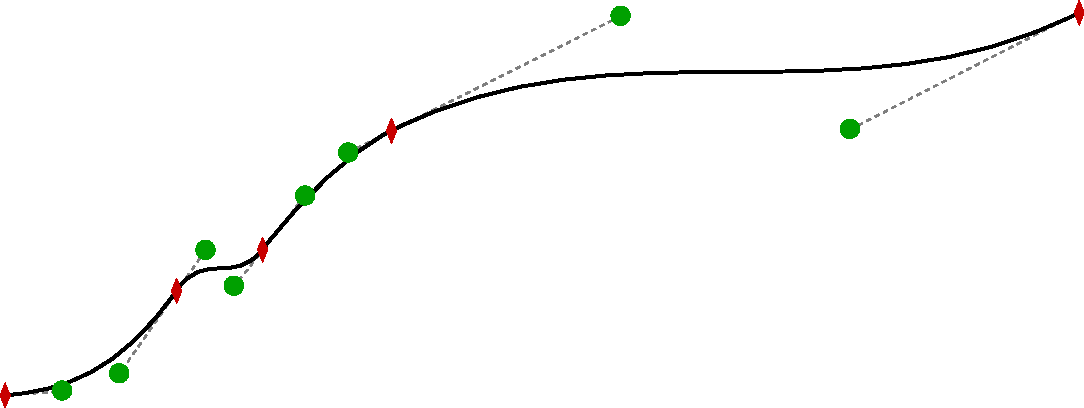
\includegraphics[width=\linewidth]{figures/chapter4/composite-bezier.pdf}
\caption{A composite cubic Bezier curve.}
\label{fig:composite-Bezier}
\end{figure}


%---search variables: time of time symbols
A real-valued variable $T$ is assigned for each new time symbol $t$ that appears in \clingo{equal()}, \clingo{lessThan()}, or a stop event.
%
These are the only new time symbols that are potentially consequential to traffic rules, due to our custom choice rules (in Step 2) for perceptible order.%
\footnote{This restriction reduces the number of search variables and constraints, thus simplifies the SMT search problem significantly.}
%
The rest of the new time symbols are for lane events (that were not consequential to the right-of-way violations,) and their numerical value can be determined from their car's time-to-distance-travelled mapping (after it is found) and their distance.


%---composite Bezier curves introduction
We use piecewise cubic polynomial functions in the form of composite Bezier curves to represent the distance travelled by a car as function of time.
%
The coefficients of the polynomials are in the form of \emph{control points}.
%
The crucial property for our purposes is the \emph{local control property}.
%
That is, changing a control point, affects the function only locally.
%
For example, if an SMT solver has fixed the first few control points to control the speed of a car before entering the intersection, it can change later control points, say for inside the intersection, without invalidating the speed before entrance.
%
\emph{Cubic} Bezier curves have four control points.
%
The first and the last control points are \emph{interpolating} points, meaning that the curve passes through those points.
%
The second and the third points determine the slope of the curve at the first and the last point, respectively.
%
See Figure~\ref{fig:bezier} for examples.
%
A \emph{composite} Bezier curve is a sequence of Bezier curves where the end of each segment is the start of the next segment.
%
See Figure~\ref{fig:composite-Bezier} for an example.
%
The red diamonds and green dots indicate the interpolating and intermediate control points of the segments, respectively.
%
See \cite{Farin.2002} for more on Bezier curves.


%---search variables: time-to-distance mapping
The representation of a time-to-distance mapping is as follows.
%
For each pair of time variables $T_i, T_{i+1}$ of a car that are consecutive (with respect to the \clingo{realLTE()} order between their time symbols), a cubic Bezier segment is instantiated.
%
The four control points of the segment are $(T_i, d_i)$, $(T_i + \frac{T_{i+1}-T_i}{3}, d_{i,1})$, $(T_i + \frac{2(T_{i+1}-T_i)}{3}, d_{i,2})$, and $(T_{i+1}, d_{i+1})$.
%
Here $d_{i,1}$ and $d_{i,2}$ are real-valued variables;
$d_i$ is the travelled distance for the event corresponding to $T_i$ which is a determined number for a lane event, and a real-valued variable otherwise; and $d_{i+1}$ is defined similarly.
%
Furthermore, the first segment has the control points $(0, 0)$, $(\frac{T_1}{3}, d_{0,1})$, $(\frac{2T_1}{3}, d_{0,2})$, $(T_1, d_1)$; and the last segment has the control points $(T_n, d_n)$, $(T_n + \frac{T_M-T_n}{3}, d_{n,1})$, $(T_n + \frac{2(T_M-T_n)}{3}, d_{n,2})$, $(T_M, d_M)$, where is $T_M$ is the duration of the scenario, and $d_M$ is the total travelled distance of the car as determined in Step 1.


%---temporal constraints
The perceptible order constraint is specified as follows.
%
For a time symbol $t$, let $v(t)$ be its numerical value if $t$ is for an old event, otherwise let $v(t)$ be its assigned time variable $T$.
%
Now for any time variable $S$, if \clingo{equal(s,t)} or \clingo{equal(t,s)} then we require $|S-v(t)| < m$, if \clingo{lessThan(s,t)} then we require $m \leq v(t)-S$, and if \clingo{lessThan(t,s)} then we require $m \leq S-v(t)$, where $m$ is the minimum perceptible time difference.
%
As for temporal order, if \clingo{realLTE(s,t)} and \clingo{not realLTE(t,s)} then we require $S < v(t)$.
%
Similarly if \clingo{realLTE(t,s)} and \clingo{not realLTE(s,t)} then we require $v(t) < S$.

%---no new lane events
\begin{figure}% >>>
  \centering
  \begin{minipage}[t]{.495\linewidth}
    {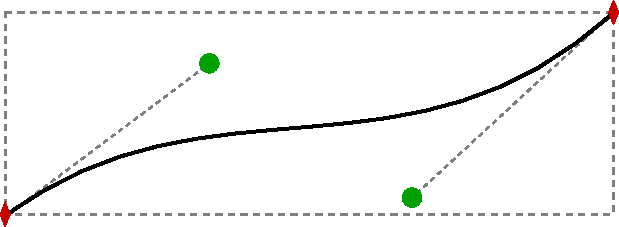
\includegraphics[width=\linewidth]{figures/chapter4/bezier-monotonic.pdf}}%
    \subcaption{Curve bounded between the heights of endpoints.}
  \end{minipage}%
  \hfill
  \begin{minipage}[t]{.495\linewidth}
    {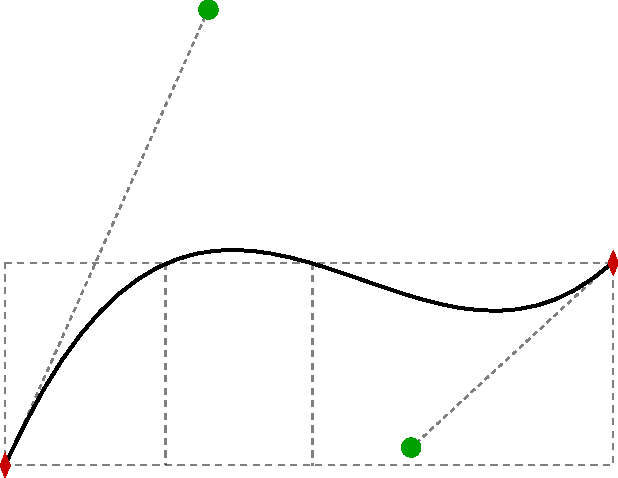
\includegraphics[width=\linewidth]{figures/chapter4/bezier-nonmonotonic.pdf}}%
    \subcaption{Curve created a new lane event at a vertical dotted line.}
  \end{minipage}%
  \caption{No-new-lane-event constraint.}\label{fig:bezier}%
\end{figure}% <<<

%---no new lane events
We must ensure that the Bezier interpolation does not create new lane events consequential to right-of-way.
%
In Figure~\ref{fig:bezier}(b), suppose that the right endpoint of the curve represents entering a lane.
%
The height of the curve reaches the height of the right endpoint at the vertical dotted lines which implies that the car enters the lane sooner than intended.
%
We prevent new lane events by requiring that the heights of the intermediate control points be between the heights of the endpoints.
%
$$ d_i \leq d_{i,1} \leq d_{i+1}, \quad d_i \leq d_{i,2} \leq d_{i+1}.
$$
%
Then the convex hull property implies that the whole interpolated Bezier segment stays within its endpoint heights, e.g. as in Figure~\ref{fig:bezier}(a).





%---longitudinal acceleration bounds
The longitudinal acceleration constraints are as follows.
%
The second derivative of a cubic polynomial is linear so its extrema over a closed interval are achieved at the endpoints.
%
For an interval $[T_i, T_{i+1}]$, the second derivatives at endpoints are
$$
a_i = \frac{6(d_i-2d_{i,1}+d_{i,2})}{(T_{i+1}-T_i)^2}, \quad
a_{i+1} = \frac{6(d_{i,1}-2d_{i,2}+d_{i+1})}{(T_{i+1}-T_i)^2}.
$$
%
Therefore, if $a_m$ and $a_M$ are respectively the minimum and maximum bounds on longitudinal acceleration, we require
$$ a_m \leq a_i \leq a_M, \quad a_m \leq a_{i+1} \leq a_M.
$$
%
These inequalities are quadratic since we can remove the fractions by multiplying the inequalities by $(T_{i+1}-T_i)^2$.


%---smooth speed
Our scenarios do not include collision events, as discussed in \S\ref{sec:problem}, so the speed of a car, i.e. the slope of the time-distance curve, must be continuous.
%
Each segment of a composite Bezier curve is a smooth function since it is a polynomial.
%
At interpolating points between two consecutive segments, we force the slopes on both sides to be equal with the quadratic equation
$$ \frac{d_i-d_{i-1,2}}{T_i-T_{i-1}} = \frac{d_{i,1}-d_i}{T_{i+1}-T_i}.
$$

%---stop events constraints
A stop event implies a constraint on the instantaneous speed of the car.
%
If $T_i$ is a time variable for a stop event, we require the instantaneous speed at $T_i$ to be within a threshold $v_{stop} \geq 0$:
$$ \frac{d_{i,1}-d_i}{\frac{1}{3}(T_{i+1}-T_i)} \leq v_{stop} $$
%
If a car violates a stop sign, we require the instantaneous speed between arrival at and entrance to the intersection to be at least a threshold $v_{run}$ where $v_{run} > v_{stop}$.
%
It is sufficient to force the slope to not have a local minimum over the interval, and the slopes at the endpoints to be at least $v_{run}$.
%
For the slope of the function to not have a local minimum over the interval, the second derivative should not change from negative to positive:
$$
\lnot (a_i < 0 \;\land\; a_{i+1} > 0)
$$
which is equivalent to the linear inequalities
$$ d_i-2d_{i,1}+d_{i,2} \geq 0 \;\lor\; d_{i,1}-2d_{i,2}+d_{i+1} \leq 0.
$$
%
The lower bound on endpoint slopes are specified with the linear inequalities
$$ \frac{d_{i,1}-d_i}{\frac{1}{3}(T_{i+1}-T_i)} \geq v_{run}, \quad \frac{d_{i+1}-d_{i,2}}{\frac{1}{3}(T_{i+1}-T_i)} \geq v_{run}.
$$

%---no SMT solution
If the SMT solver returns `unsatisfiable', Step 3 is repeated with the next ASP solution, if any.
%
If no ASP solution remains, the algorithm returns with no solutions.

%---SMT solution
If the SMT solver returns a solution, i.e. coordinates of the control points, we can sample points on the time-distance curves using the standard de Casteljau algorithm for Bezier curve computation.
%
This gives the time-to-distance-travelled mapping.
%
Composing this with the travelled distance at each pose, we get the pose at each time.